\documentclass[handout,aspectratio=169]{beamer}
\usepackage[english]{babel}
\usepackage{metalogo}
\usepackage{listings}
\usepackage{fontspec}
\usepackage{tikz}
\usepackage{graphicx}
\usepackage{subcaption}
%%%%%%%%%%%%%%%%%%%%%%%%%%%%%%%%%%%%%%%%%%%%%%%%%%%%%%%%%%%%%%%%%%%%%%%%%%%%%%%%%%%%%%%%
%%%%%%%%%%%%%%%%%%%%%%%%%%%%%%%%%%%%%%%%%%%%%%%%%%%%%%%%%%%%%%%%%%%%%%%%%%%%%%%%%%%%%%%%
%%%%%%%%%%%%%%%%%%%%%%%%%%%%%%%%%%%%%%%%%%%%%%%%%%%%%%%%%%%%%%%%%%%%%%%%%%%%%%%%%%%%%%%%
\usepackage{xcolor}
\definecolor{BK}{HTML}{3b3838}
\definecolor{Blue}{RGB}{88, 105, 225}
\newcommand{\BK}[1]{\color{BK} #1}
\newcommand{\URed}[1]{\color{URed} #1}
\newcommand{\white}[1]{\color{white} #1}
\newcommand{\Orange}[1]{\color{QOrange} #1}
\newcommand{\blue}[1]{\color{blue} #1}
\newcommand{\Blue}[1]{\color{Blue} #1}
\newcommand{\red}[1]{\color{red} #1}
\newcommand{\gray}[1]{\color{gray} #1}
\newcommand{\orange}[1]{\color{orange} #1}
\usepackage{accents}
\newcommand\thickbar[1]{\accentset{\rule{.4em}{.8pt}}{#1}}
\newcommand{\ubar}[1]{\underaccent{\bar}{#1}}
\newcommand{\hatbar}[1]{\bar{\hat{#1}}}
\newcommand{\hatubar}[1]{\underaccent{\bar}{\hat{#1}}}
\newcommand{\ul}[1]{\underline{#1}}
\newcommand{\ol}[1]{\overline{#1}}
%%%%%%%%%%%%%%%%%%%%%%%%%%%%%%%%%%%%%%%%%%%%%%%%%%%%%%%%%%%%%%%%%%%%%%%%%%%%%%%%%%%%%%%%
\newcommand{\bO}[1]{\bf \Orange #1}
%%%%%%%%%%%%%%%%%%%%%%%%%%%%%%%%%%%%%%%%%%%%%%%%%%%%%%%%%%%%%%%%%%%%%%%%%%%%%%%%%%%%%%%%
%%%%%%%%%%%%%%%%%%%%%%%%%%%%%%%%%%%%%%%%%%%%%%%%%%%%%%%%%%%%%%%%%%%%%%%%%%%%%%%%%%%%%%%%
\newcommand{\YBox}[3]{
\begin{center}
\begin{minipage}{#1\linewidth}
\begin{exampleblock}{#2}
    #3
\end{exampleblock}
\end{minipage}
\end{center}
}

\newcommand{\OBox}[3]{
\begin{center}
\begin{minipage}{#1\linewidth}
\begin{block}{#2}
    #3
\end{block}
\end{minipage}
\end{center}
}

\newcommand{\Columns}[4]{
\begin{columns}
\begin{column}{#1\textwidth}
#2
\end{column}
\begin{column}{#3\textwidth}  %%<--- here
#4
\end{column}
\end{columns}
}
\input{commands_math}
\usetheme{Nord}
%%%%% \setmainfont{}
\setmainfont{Montserrat}
\setsansfont{Andika New Basic}
\setmonofont{DejaVu Sans Mono}

%%%%%%%%%%%%%%%%%%%%%%%%%%%%%%%%%%%%%%%%%%%%%%%%%%%%%%%%%%%%%%%%%%%%%%%%%%%%%%%%%%%%%%%%
%%%%%%%%%%%%%%%%%%%%%%%%%%%%%%%%%%%%%%%%%%%%%%%%%%%%%%%%%%%%%%%%%%%%%%%%%%%%%%%%%%%%%%%%
\newcommand{\bs}{

\bigskip

}
\newcommand{\ms}{

\medskip

}
%%%%%%%%%%%%%%%%%%%%%%%%%%%%%
\usepackage{tcolorbox}
\newtcolorbox{mybox}{width=9cm, left=0mm,right = 0mm,top=1mm,bottom=1mm,boxsep=0mm}
\newtcolorbox{myboxL}{width=15cm, left=0mm,right = 0mm,top=1mm,bottom=1mm,boxsep=0mm}
\newtcolorbox{mybox1}{width=5.5cm, left=0mm,right = 0mm,top=1mm,bottom=1mm,boxsep=0mm,colback=BK, coltext=QOrange}

\newtcolorbox{mybox2}{width=12cm, left=0mm,right = 0mm,top=1mm,bottom=1mm,boxsep=0mm,colback=BK, coltext=QOrange}

\newtcolorbox{mybox3}{width=3cm, left=0mm,right = 0mm,top=1mm,bottom=1mm,boxsep=0mm,colback=BK, coltext=QOrange}

\newtcolorbox{mybox4}{width=11cm, left=1mm,right = 1mm,top=1mm,bottom=1mm,boxsep=0mm,colback=BK, coltext=QOrange}
%%%%%%%%%%%%%%%%%%%%%%%%%%%%%%%%%%%%%%%%%%%%%%%%%%%%%%%%%%%%%%%%%%%%%%%%%%%%%%%%%%%%%%%%
%%%%%%%%%%%%%%%%%%%%%%%%%%%%%%%%%%%%%%%%%%%%%%%%%%%%%%%%%%%%%%%%%%%%%%%%%%%%%%%%%%%%%%%%

\usepackage{amsmath}
\graphicspath{{figs/fig00/}}
%-----------------
%	TITLE
%-----------------
\title{
Chapter 03: Filtering
}
\author{\bf Notes by Kumar Anurag}
\date{}

%-----------------
%	SUBTITLE
%-----------------
\subtitle{
Probabilistic Artificial Intelligence
}

\begin{document}

%-----------------
%	TITLE PAGE
%-----------------
{\usebackgroundtemplate{\includegraphics[width=\paperwidth]{chapter_figs/01_figs/titlepic.png}}
	\begin{frame}[plain,noframenumbering]
		\maketitle
	\end{frame}}


%-----------------------
%	PRESENTATION SLIDES
%-----------------------

\begin{frame}{The Story of Blindfolded Robot}

\textbf{Imagine:}

\begin{columns}
    \column{0.6\textwidth}
\begin{itemize}
  \item A robot is navigating down a hallway, but it’s \textbf{blindfolded}.
  \item It can’t see where it is — it only has a noisy distance sensor and a map of the hallway.
  \item At each step, it must decide:
  \begin{itemize}
    \item Where it \textit{thinks} it is,
    \item How to move next,
    \item And how to adjust based on new noisy sensor readings.
  \end{itemize}
\end{itemize}

\vspace{1em}
\textbf{The robot’s challenge is exactly what filtering solves:}
\begin{quote}
  \centering
  \emph{“Estimate where you are over time — with incomplete and uncertain information.”}
\end{quote}

    \column{0.4\textwidth}
    \begin{center}
		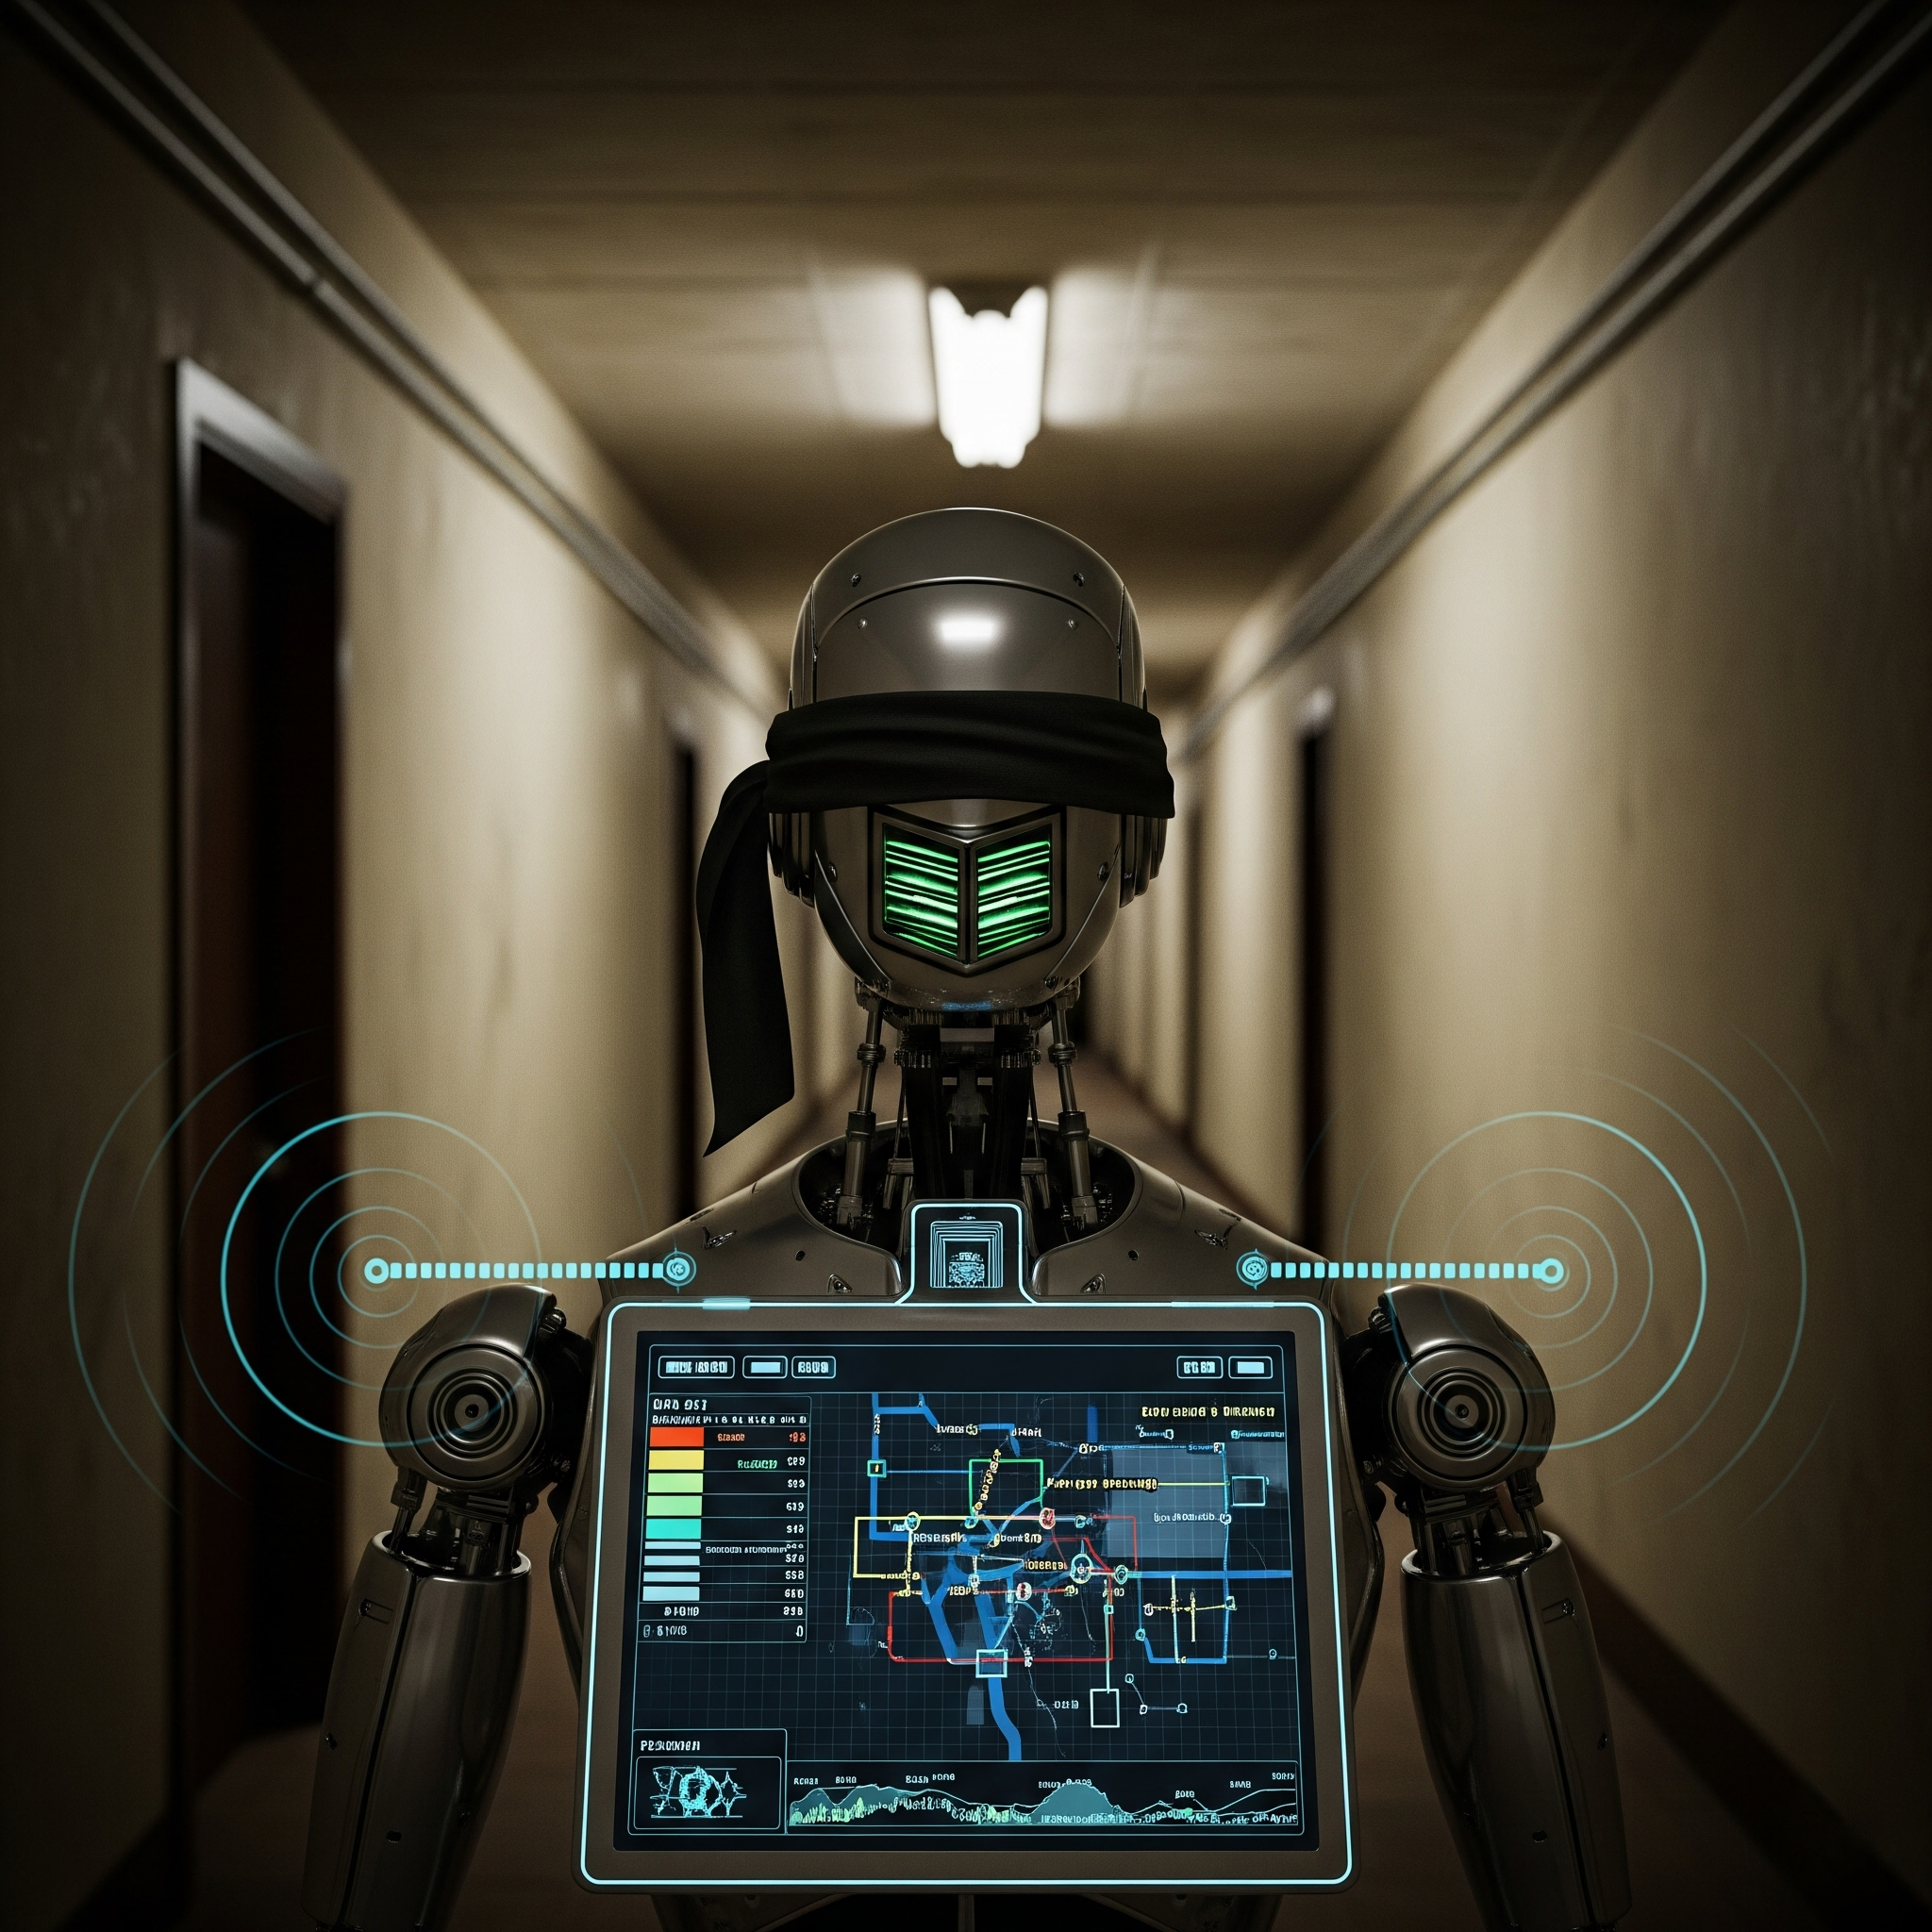
\includegraphics[width=\linewidth]{chapter_figs/03_figs/blind_folded_robot.png}
\end{center}
\end{columns}


\end{frame}

\begin{frame}{What is Filtering? The Core Problem}

\textbf{Filtering} is about estimating the \textbf{hidden state} of a system over time, using a stream of noisy observations.

\vspace{0.8em}
\begin{block}{Why it’s harder than regular regression}
\begin{itemize}
  \item The unknown (state) keeps changing.
  \item The observations are noisy and only partially informative.
  \item We must update our estimate \textit{as new data arrives}.
\end{itemize}
\end{block}

\vspace{0.8em}
\textbf{We need:}
\begin{itemize}
  \item A \textbf{dynamics model}: How the state evolves over time.
  \item An \textbf{observation model}: How observations relate to the state.
\end{itemize}

\vspace{0.8em}
\textbf{Applications:}
\begin{itemize}
  \item Self-driving cars, speech recognition, finance, robotics, weather prediction...
\end{itemize}

\end{frame}

\begin{frame}{State Space Models (SSMs)}

\textbf{Let’s formalize the blindfolded robot’s world.}

\vspace{1em}
\begin{itemize}
  \item \textbf{Hidden States:} \( X_t \in \mathbb{R}^d \)
  \begin{itemize}
    \item The robot’s true position, speed, or internal state at time \( t \).
    \item Not directly visible — we want to estimate it!
  \end{itemize}

  \vspace{0.6em}
  \item \textbf{Observations:} \( Y_t \in \mathbb{R}^m \)
  \begin{itemize}
    \item Sensor readings at time \( t \).
    \item Noisy, partial glimpses of the hidden state.
  \end{itemize}

  \vspace{0.6em}
  \item \textbf{Goal:} Given observations up to time \( t \), i.e. \( Y_{1:t} \),
  \begin{itemize}
    \item Estimate the current state \( X_t \).
    \item Sometimes even forecast future states \( X_{t+1}, X_{t+2}, \dots \)
  \end{itemize}
\end{itemize}

\vspace{1em}
\begin{block}{Key Idea}
SSMs capture how the world evolves (\textit{state transition}) and how we perceive it (\textit{observation model}).
\end{block}

\end{frame}

\begin{frame}{Bayesian Filtering: The Big Picture}

\textbf{Our Goal:} Maintain a belief about the hidden state \( X_t \) as we receive observations \( Y_{1:t} \).

\vspace{1em}
\begin{block}{Recursive Bayesian Estimation}
At every time step, we perform two key operations:
\end{block}

\vspace{0.5em}
\textbf{1. Prediction (Time Update):}
\[
p(X_{t} \mid Y_{1:t-1}) = \int p(X_t \mid X_{t-1}) \, p(X_{t-1} \mid Y_{1:t-1}) \, dX_{t-1}
\]

\vspace{0.5em}
\textbf{2. Update (Measurement Correction):}
\[
p(X_t \mid Y_{1:t}) \propto p(Y_t \mid X_t) \, p(X_t \mid Y_{1:t-1})
\]

\vspace{0.5em}
\textbf{Repeat:} These steps are performed in a loop as new data arrives.
\end{frame}

\begin{frame}{Figure 3.1: How Bayesian Filtering Works}

\begin{columns}
\column{0.4\textwidth}
\includegraphics[width=\linewidth]{chapter_figs/03_figs/3_1.png} 

\column{0.6\textwidth}
\textbf{Explanation:}
\begin{itemize}
  \item The \textbf{true world state} evolves over time: \( \text{world}_t \to \text{world}_{t+1} \).
  \item The agent perceives each state through noisy data: \( D_t, D_{t+1} \).
  \item Based on its observations \( D_{1:t} \), it maintains a belief (posterior) over the hidden variables: 
  \[
  p(\theta \mid D_{1:t})
  \]
  \item At each time step, the agent:
  \begin{enumerate}
    \item \textbf{Updates} its belief using new data.
    \item \textbf{Predicts} the next state of the world.
  \end{enumerate}
\end{itemize}
\end{columns}

\begin{block}{Core Idea}
Filtering is the cycle of \textit{observe \rightarrow update belief \rightarrow  predict \rightarrow  repeat}.
\end{block}

\end{frame}

\begin{frame}{Introducing the Kalman Filter}

\textbf{Kalman Filter:} A powerful, tractable solution to the filtering problem — when everything is linear and Gaussian.


\begin{block}{Assumptions}
\begin{itemize}
  \item Initial state: Gaussian prior over \( X_0 \)
  \item Dynamics model: Linear with Gaussian process noise
  \item Observation model: Linear with Gaussian measurement noise
\end{itemize}
\end{block}


\textbf{Why it's useful:}
\begin{itemize}
  \item The belief at each step — the posterior \( p(X_t \mid Y_{1:t}) \) — stays Gaussian.
  \item All filtering steps (prediction and update) have closed-form analytical solutions.
\end{itemize}


\begin{block}{Key Insight}
\textit{Linear-Gaussian systems allow exact, recursive inference — no sampling or approximations needed.}
\end{block}

\end{frame}

\begin{frame}{Kalman Filter: Formal Definition}

\textbf{The Kalman Filter is defined by three components:}

\begin{enumerate}
  \item \textbf{Initial State (Prior Belief):}
  \[
    X_0 \sim \mathcal{N}(\mu_0, \Sigma_0) \tag{3.1}
  \]

  \item \textbf{State Transition Model (Dynamics):}
  \[
    X_{t+1} = F X_t + \varepsilon_t, \quad \varepsilon_t \sim \mathcal{N}(0, \Sigma_x) \tag{3.2}
  \]
  \begin{itemize}
    \item \( F \): State transition matrix (\( d \times d \))
    \item \( \varepsilon_t \): Process noise (may include drift; zero-mean assumed here)
  \end{itemize}

  \item \textbf{Observation Model (Sensor):}
  \[
    Y_t = H X_t + \eta_t, \quad \eta_t \sim \mathcal{N}(0, \Sigma_y) \tag{3.3}
  \]
  \begin{itemize}
    \item \( H \): Observation matrix (\( m \times d \))
    \item \( \eta_t \): Measurement noise
  \end{itemize}
\end{enumerate}

\textbf{Note:} \( F, H, \Sigma_x, \Sigma_y \) are assumed to be known (can be time-varying).

\end{frame}

\begin{frame}{Graphical Model and Conditional Independencies}

\begin{columns}
    \column{0.7\textwidth}
    \textbf{Kalman Filter as a Probabilistic Graphical Model:}
\begin{itemize}
  \item Hidden state sequence: \( X_1 \rightarrow X_2 \rightarrow X_3 \rightarrow \dots \)
  \item Each \( X_t \) emits an observation \( Y_t \)
\end{itemize}

    \column{0.3\textwidth}
    \includegraphics[width=\textwidth]{chapter_figs/03_figs/3_2.png} 
\end{columns}

\begin{block}{Conditional Independencies}
\begin{itemize}
  \item \textbf{Markov Property (Eq. 3.4):}
  \[
    X_{t+1} \perp \!\!\! \perp X_{1:t-1}, Y_{1:t-1} \mid X_t
  \]
  Future state depends only on the current state.
  \end{itemize}
\end{block}
\end{frame}

\begin{frame}{Graphical Model and Conditional Independencies}
\begin{block}{Conditional Independencies}
\begin{itemize}
  \item \textbf{Observation Dependence (Eq. 3.5):}
  \[
    Y_t \perp \!\!\! \perp X_{1:t-1} \mid X_t
  \]
  Observation depends only on the current state.

  \item \textbf{Observation Independence (Eq. 3.6):}
  \[
    Y_t \perp \!\!\! \perp Y_{1:t-1} \mid X_{t-1}
  \]
  Given the past state, current observation is independent of past observations.
\end{itemize}
\end{block}

\end{frame}

\begin{frame}{The Goal: Online Recursive Estimation}

\textbf{What we want:}
\begin{itemize}
  \item At each time \( t \), compute the belief:
  \[
    p(X_t \mid Y_{1:t})
  \]
  \item Without re-processing all past data from scratch!
\end{itemize}


\textbf{Why Online?}
\begin{itemize}
  \item Observations arrive sequentially in real-time.
  \item We need to update our estimate efficiently and recursively.
  \item No need to store all \( Y_{1:t} \) — just the current posterior!
\end{itemize}


\begin{block}{Recursive Filtering Loop}
\begin{enumerate}
  \item Predict: Use dynamics model to forecast next state.
  \item Update: Incorporate new observation.
  \item Repeat...
\end{enumerate}
\end{block}


\textit{This is the essence of recursive Bayesian estimation.}

\end{frame}

\begin{frame}{Algorithm: Bayesian Filtering}

\includegraphics[width=0.8\textwidth]{chapter_figs/03_figs/algorithm.png} 
\end{frame}

\begin{frame}{Bayesian Filtering: Prediction and Conditioning}
\begin{block}{1. Conditioning (Update Step)}
\textit{Incorporate new observation \( Y_t \) to refine belief about \( X_t \)}
\[
p(X_t \mid Y_{1:t}) \propto p(Y_t \mid X_t) \cdot p(X_t \mid Y_{1:t-1}) \tag{3.8}
\]
\begin{itemize}
  \item Combines the prior (predicted) belief with the new observation.
  \item Uses Bayes’ Rule.
\end{itemize}
\end{block}
\end{frame}

\begin{frame}{Bayesian Filtering: Prediction and Conditioning}
\begin{block}{2. Prediction (Time Update Step)}
\textit{Project the belief forward to estimate \( X_{t+1} \)}
\[
p(X_{t+1} \mid Y_{1:t}) = \int p(X_{t+1} \mid X_t) \cdot p(X_t \mid Y_{1:t}) \, dX_t \tag{3.9}
\]
\begin{itemize}
  \item Uses the transition model to forecast the next state.
  \item Allows filtering to continue over time.
\end{itemize}
\end{block}

\end{frame}

\begin{frame}{Deriving the Conditioning (Update) Step}

\textbf{Goal:} Update belief about current state given a new observation:
\[
p(X_t \mid Y_{1:t}) = \text{posterior}
\]

\textbf{Start from:}
\[
p(X_t \mid Y_{1:t}) = p(X_t \mid Y_t, Y_{1:t-1})
\]

\textbf{Apply Bayes’ Rule:}
\[
p(X_t \mid Y_{1:t}) \propto p(Y_t \mid X_t, Y_{1:t-1}) \cdot p(X_t \mid Y_{1:t-1})
\]

\textbf{Use Conditional Independence (Eq. 3.6):}
\[
Y_t \perp Y_{1:t-1}, X_{1:t-1} \setminus X_t \mid X_t \Rightarrow p(Y_t \mid X_t, Y_{1:t-1}) = p(Y_t \mid X_t)
\]

\textbf{Final form:}
\[
p(X_t \mid Y_{1:t}) \propto p(Y_t \mid X_t) \cdot p(X_t \mid Y_{1:t-1}) \tag{3.8}
\]

\begin{block}{Interpretation}
\textbf{Posterior} \( \propto \) \textbf{Likelihood} \( \times \) \textbf{Prior}
\end{block}

\end{frame}

\begin{frame}{Deriving the Prediction Step}

\textbf{Goal:} Predict the next state before the next observation arrives:
\[
p(X_{t+1} \mid Y_{1:t})
\]

\textbf{Step 1: Apply marginalization}
\[
p(X_{t+1} \mid Y_{1:t}) = \int p(X_{t+1}, X_t \mid Y_{1:t}) \, dX_t
\]

\textbf{Step 2: Use the product rule}
\[
= \int p(X_{t+1} \mid X_t, Y_{1:t}) \cdot p(X_t \mid Y_{1:t}) \, dX_t
\]

\textbf{Step 3: Apply the Markov Property (Eq. 3.4):}
\[
X_{t+1} \perp Y_{1:t} \mid X_t \Rightarrow p(X_{t+1} \mid X_t, Y_{1:t}) = p(X_{t+1} \mid X_t)
\]

\textbf{Final Result:}
\[
p(X_{t+1} \mid Y_{1:t}) = \int p(X_{t+1} \mid X_t) \cdot p(X_t \mid Y_{1:t}) \, dX_t \tag{3.9}
\]

\end{frame}

\begin{frame}{Kalman Filter: The Prediction Step}

\textbf{Given:} Posterior at time \( t \):
\[
X_t \mid Y_{1:t} \sim \mathcal{N}(\mu_t, \Sigma_t)
\]

\textbf{We want:} Predictive belief for time \( t+1 \):
\[
X_{t+1} \mid Y_{1:t} \sim \mathcal{N}(\hat{\mu}_{t+1}, \hat{\Sigma}_{t+1})
\]

\textbf{Apply the transition model:}
\[
X_{t+1} = F X_t + \varepsilon_t, \quad \varepsilon_t \sim \mathcal{N}(0, \Sigma_x)
\]

\begin{block}{Predicted Mean (Eq. 3.20)}
\[
\hat{\mu}_{t+1} = F \mu_t
\]
\end{block}

\begin{block}{Predicted Covariance (Eq. 3.21)}
\[
\hat{\Sigma}_{t+1} = F \Sigma_t F^\top + \Sigma_x
\]
\end{block}
\end{frame}

\begin{frame}{Kalman Filter: The Update Step}

\textbf{We have:}
\begin{itemize}
  \item Prior prediction: \( X_{t+1} \mid Y_{1:t} \sim \mathcal{N}(\hat{\mu}_{t+1}, \hat{\Sigma}_{t+1}) \)
  \item New observation: \( Y_{t+1} = H X_{t+1} + \eta_{t+1}, \; \eta_{t+1} \sim \mathcal{N}(0, \Sigma_y) \)
\end{itemize}

\begin{block}{Kalman Gain (Eq. 3.18d)}
\[
K_{t+1} = \hat{\Sigma}_{t+1} H^\top \left( H \hat{\Sigma}_{t+1} H^\top + \Sigma_y \right)^{-1}
\]
\end{block}

\begin{block}{Updated Mean (Eq. 3.18b)}
\[
\mu_{t+1} = \hat{\mu}_{t+1} + K_{t+1} \left( Y_{t+1} - H \hat{\mu}_{t+1} \right)
\]
\end{block}

\begin{block}{Updated Covariance (Eq. 3.18c)}
\[
\Sigma_{t+1} = \left( I - K_{t+1} H \right) \hat{\Sigma}_{t+1}
\]
\end{block}

\end{frame}

\begin{frame}{Example 3.4 – Random Walk in 1D}

\textbf{System Setup:}

\begin{itemize}
  \item \textbf{State:} \( X_t \in \mathbb{R} \) (position on a line)
  \item \textbf{Motion Model:}
  \[
    X_{t+1} = X_t + \varepsilon_t, \quad \varepsilon_t \sim \mathcal{N}(0, \sigma_x^2)
  \]
  \item \textbf{Sensor Model:}
  \[
    Y_t = X_t + \eta_t, \quad \eta_t \sim \mathcal{N}(0, \sigma_y^2)
  \]
  \item \textbf{Initial Belief:} \( X_0 \sim \mathcal{N}(\mu_0, \sigma_0^2) \)
\end{itemize}

\textbf{Kalman Filter simplifies to 1D:}

\begin{itemize}
  \item Prediction and update equations become scalar operations.
  \item Still recursive!
  \item Posterior: \( X_t \mid Y_{1:t} \sim \mathcal{N}(\mu_t, \sigma_t^2) \)
\end{itemize}

\begin{block}{Key Idea}
Even this simple setup captures the trade-off between motion uncertainty and noisy observations.
\end{block}

\end{frame}

\begin{frame}{Random Walk – 1D Kalman Update (Eq. 3.13)}

\textbf{Recall:}
\begin{itemize}
  \item Prior at time \( t \): \( X_t \mid Y_{1:t} \sim \mathcal{N}(\mu_t, \sigma_t^2) \)
  \item Prediction for \( t+1 \): 
  \[
    X_{t+1} \mid Y_{1:t} \sim \mathcal{N}(\mu_{t+1}, \sigma_{t+1}^2 )
  \]
  \item Observation: \( Y_{t+1} = X_{t+1} + \eta_{t+1}, \; \eta_{t+1} \sim \mathcal{N}(0, \sigma_y^2) \)
\end{itemize}

\textbf{Update step (Eq. 3.13):}
\[
\mu_{t+1} = \frac{\sigma_y^2 \mu_t + (\sigma_t^2 + \sigma_x^2) Y_{t+1}}{\sigma_t^2 + \sigma_x^2 + \sigma_y^2}
\]

\[
\sigma_{t+1}^2 = \frac{(\sigma_t^2 + \sigma_x^2) \sigma_y^2}{\sigma_t^2 + \sigma_x^2 + \sigma_y^2}
\]

\end{frame}

\begin{frame}{Kalman Gain \( \lambda \) and Equivalent Update Forms}

\textbf{Kalman Gain in 1D (Eq. 3.14):}
\[
\lambda = \frac{\sigma_t^2 + \sigma_x^2}{\sigma_t^2 + \sigma_x^2 + \sigma_y^2}
\]

\vspace{1em}
\textbf{Updated Mean (Eq. 3.15, 3.16):}
\[
\mu_{t+1} = (1 - \lambda) \mu_t + \lambda Y_{t+1} \tag{3.15}
\]
\[
= \mu_t + \lambda (Y_{t+1} - \mu_t) \tag{3.16}
\]

\vspace{0.8em}
\textbf{Updated Variance (Eq. 3.17):}
\[
\sigma_{t+1}^2 = (1 - \lambda)(\sigma_t^2 + \sigma_x^2) = \lambda \sigma_y^2
\]


\end{frame}

\begin{frame}{Bayesian Linear Regression as a Kalman Filter}

\textbf{Problem Setup:}
\begin{itemize}
  \item We want to estimate a fixed but unknown weight vector \( w^* \in \mathbb{R}^d \)
  \item Observations arrive sequentially: \( (x_t, y_t) \), where
  \[
    y_t = x_t^\top w^* + \eta_t, \quad \eta_t \sim \mathcal{N}(0, \sigma_n^2)
  \]
\end{itemize}

\vspace{0.8em}
\textbf{Kalman Filter Interpretation:}
\begin{itemize}
  \item Hidden state: \( X_t = w^* \) (constant!)
  \item Transition model: \( X_{t+1} = X_t + 0 \) \rightarrow no process noise \rightarrow \( \Sigma_x = 0 \)
  \item Sensor model:
  \[
    Y_t = x_t^\top X_t + \eta_t
  \]
  \item Observation matrix: \( H_t = x_t^\top \)
\end{itemize}

\begin{block}{Connection}
\textit{Online Bayesian Linear Regression is Kalman Filtering with constant hidden state.}
\end{block}

\end{frame}

\begin{frame}{Bayesian Smoothing: LookingBackWithMoreInfo}

\textbf{Filtering:} Estimates the current state using data \textbf{up to} time \( t \)
\[
p(X_k \mid Y_{1:k}) \quad \text{(for } k = t\text{)}
\]

\textbf{Smoothing:} Estimates a \textbf{past} state \( X_k \) using all data \textbf{up to a later time} \( t \)
\[
p(X_k \mid Y_{1:t}) \quad \text{where } k < t
\]

\textbf{Why Smooth?}
\begin{itemize}
  \item Gives more accurate estimate of \( X_k \) using future evidence.
  \item Useful in offline settings (e.g., analyzing recorded sensor data).
\end{itemize}
\end{frame}

\begin{frame}{Bayesian Smoothing: LookingBackWithMoreInfo}
\textbf{Key Equation (Eq. 3.10):} $$p(x_k \mid y_{1:t}) \propto p(x_k \mid y_{1:k}) \cdot p(y_{k+1:t} \mid x_k)$$
\begin{itemize}
  \item First term: filtering result
  \item Second term: likelihood of future observations
  \item Smoothing = Filtering + Backward Pass
  \item We combine past estimate with future information for better accuracy
\end{itemize}


\end{frame}

\begin{frame}{Kalman Smoothing: Fwd-Bkwd Estimation}

\textbf{Filtering:} Real-time estimate
\[
p(X_k \mid Y_{1:k}) = \text{filtering posterior}
\]

\textbf{Smoothing:} Offline refinement
\[
p(X_k \mid Y_{1:t}) = \text{smoothing posterior}, \quad k < t
\]

\vspace{1em}
\textbf{Linear-Gaussian Case:}
\begin{itemize}
  \item Both filtering and smoothing posteriors are Gaussian.
  \item Can compute smoothing efficiently using a backward recursion.
\end{itemize}
\end{frame}

\begin{frame}{Kalman Smoothing: Fwd-Bkwd Estimation}
\vspace{0.8em}
\textbf{Key Equation (Eq. 3.11):}
\[
p(x_k \mid y_{1:t}) = \mathcal{N}(\tilde{\mu}_k, \tilde{\Sigma}_k)
\]
\begin{itemize}
  \item Based on forward-filtered posterior \( p(x_k \mid y_{1:k}) \)
  \item And the backward Kalman gain, derived from transition model
\end{itemize}

\vspace{1em}
\begin{block}{Smoothing Algorithm = Filter Forward + Smooth Backward}
\textit{Also called the Forward-Backward or Two-Filter smoother.}
\end{block}

\vspace{1em}
\includegraphics[width=0.5\textwidth]{chapter_figs/03_figs/line.png}

\end{frame}









{\usebackgroundtemplate{\includegraphics[width=\paperwidth]{chapter_figs/03_figs/thankyou.png}}
	\begin{frame}[plain,noframenumbering]
	\end{frame}}



\end{document}